\documentclass[12pt,letterpaper]{article}

\usepackage{titlepic}

\usepackage[utf8]{inputenc}

\usepackage{amsmath}

\usepackage{amsfonts}

\usepackage{amssymb}

\usepackage{graphicx}

\usepackage[left=1in,right=1in,top=1in,bottom=1in]{geometry}


\usepackage{float}

\usepackage{setspace}

\author{Jonathan Zhou}

\title{Pictionary over Local Area Networks in the Java Language}



\begin{document}
\maketitle

\begin{figure}[H]
\centering
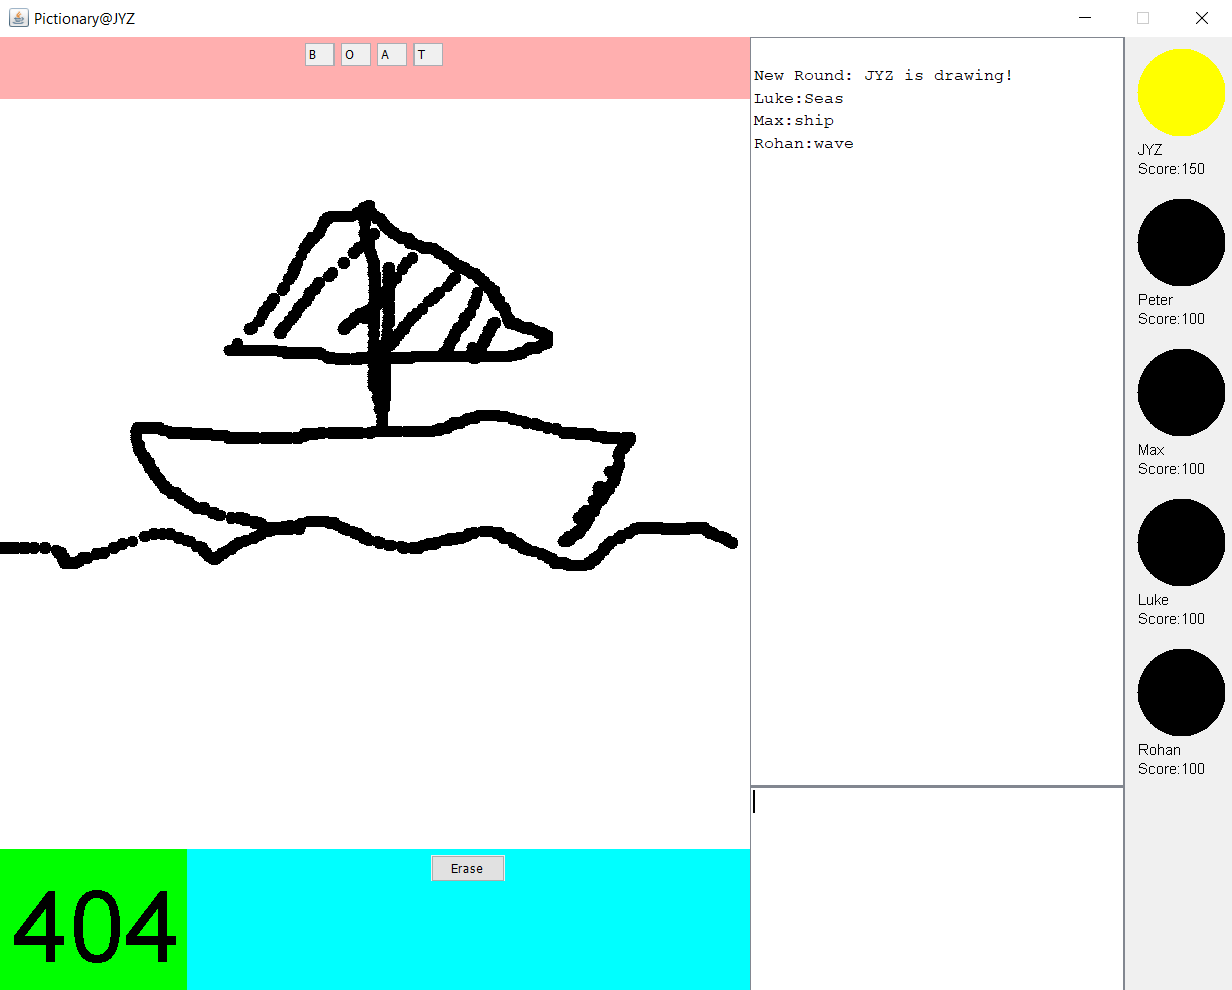
\includegraphics[width=5in]{sampleGameplay.PNG}

\caption{Sample Gameplay in Pictionary over LAN}
\end{figure}
\thispagestyle{empty}

\newpage

\doublespacing

\section*{Product Description}

\textit{Pictionary over LAN} provides an implementation of a variant of the charades-style game of Pictionary which works over networks implementing the TCP/IP protocol suite. The game follows a multiple-client server architecture. Gameplay management, control flow, and inter-client communication is directed and proxied via a networked computer which acts as a server. Players proceed to connect through a client GUI, which forms a direct connection to the server via network sockets. As game is intended to work over local area networks, most firewalls will not interfere with game operation. However, the nature of socket programming allows the game to be run across the wider internet and virtual private networks as well. Throughout game operation, the client and server concurrently pass messages (datagrams) which communicate game data (e.g. drawing, game end, new round, hint, and player messages), that results in specific action on both sides, such as the relay of said messages as well as UI and game logic updates.

Specific operation of the game is handled through multiple threads of execution. Operation begins with the invocation of the server’s main thread, with parameters for the port of connection, a word bank file path, and integer quantities for the number of rounds and the time allotted for each round. Following initialization, the server spawns a lobby thread and waits for client connections. Client connections are made via the invocation of a Pictionary welcome GUI with parameters for username, server IP, and server port. Following the entering of these parameters, the client will attempt to make a connection to the server. If this is successful, the main game client GUI will be instantiated and both a server-side client handler and a client-side server handler will be spawned. Both handlers will constantly query for game messages from this point on. After all players have joined, indicated by manually triggering an event on the server, the server will enter operation mode. Within this mode the server will loop though each of the specified rounds of operation. For each of these rounds, the server will loop through each player, assigning one as the drawer and the rest as guessers so that everyone has a chance to draw. During each round, timing threads are allocated on both the client and server sides. As players move though and guess the words correctly, they are subsequently awarded points for guessing, the less time for the guess, the more points. All players can see previously made guesses from players which have not successfully guessed the word within an in-game chat interface. A round terminates upon either the exhaustion of time, or if all players have successfully guessed the word. The player with the most points at the end of this process is determined as the winner, all clients are disconnected, and the server operation terminates.

The main goal of this game is to provide a fun game which is easy to distribute, multiplayer, and can be run on all sorts of devices. The game can be used to foster social interaction between good friends as well as strangers and create an environment in which people can spend their leisure time together without having to worry about keeping track of scores or making up words for Pictionary. The game also serves to demonstrate the capabilities of services which operate over Local Area Networks, as opposed the wider internet, saving complexity and cutting down on latency. The game is also easily modifiable and extendable due to its modular nature, for example, it could operate on a peer to peer basis with an ad hoc network. 

\textit{Pictionary over LAN} may be contrasted to two existing implementations of Pictionary: the popular online game \textit{skribbl.io} and the traditional, pen and paper style of Pictionary. The advantage of \textit{Pictionary over LAN} is in terms of convenience, openness, and privacy. The aim is to put the user in control of the game by giving them the capability to create their own server and host their own games on their own networks. The game offers greater amounts of control in terms of extensibility as well, for example custom dictionaries can be used for the words which the game will serve. This contrasts with \textit{skribbl.io}, which needs to be proxied through \textit{skribbl.io} servers and be exposed to the various layers of the internet. \textit{skribbl.io} also contains advertisements and other expensive and unnecessary UI elements. The spartan nature of \textit{Pictionary over LAN} is intentional. In addition, \textit{skribbl.io} public games often contain inappropriate content due to the user generated nature of gameplay. Though the creation of private parties, game data is still unnecessarily proxied over the wider internet. Finally, web applications such as \textit{skribbl.io} require constant internet connectivity and must contents with web-browser overheads.

In contrast to a pen a paper paradigm, \textit{Pictionary over LAN} offers much in terms convenience. With the increased proliferation of digital devices and a decline in the use of pen in paper in general, it makes sense to provide a digital implementation of this classic game. There is no need to waste large quantities of paper and set up a physical space within which Pictionary may be played. \textit{Pictionary over LAN} eliminates the need for players to serve as a moderators and tabulators for the game, as all game moderation. The game eliminates the need for tabulation of scores, which can be difficult if not impossible within classic Pictionary (especially with regards to the speed of guessing).  The computer nature of the game also provides a certain level of challenge in using a digital human input device (such as a mouse) which is not intended for drawing lines and curves.



\section*{Market Analysis}

\textit{Pictionary over LAN} is intended for children and adults ages 10 and up. Players must sociable and capable of understanding the vocabulary they are expected to draw and interpret and possess a certain level of fine motor control. As the game offers Unicode support, the Pictionary word bank is user configurable, and client usage  doesn’t require an understanding of the English language beyond the special keywords “Username” “Server IP” and “Port” (which can be easily replaced with foreign language translations) to play the game is also readily localizable.

Some network parameters (Port and IP address) must be understood at a superficial level to create a game, and configuration must be navigated for game invocation. Although configuring and instantiating a server is slightly more difficult than joining as a client, this process is still relatively simple. 

There is precedence for games such as \textit{Pictionary over LAN} within the wider game area, as evident in the proliferation and success of \textit{skribbl.io} and \textit{Quick, Draw!} along with other simple online multiplayer games. This success is extended beyond the browser as well, with various causal desktop games supporting multiplayer connectivity over LAN.

With regards to packaging and distribution the game may be distributed in both binary and source forms. The server and client would come bundled as one package. The software can either be installed to a system or be run portably (e.g. from a flash drive) for convenience. Distributions of this software can either be obtained online or from other players where the binaries may simply be copied. This allows for the game to be proliferated even when a full internet connection is not available. Server and client versions should be generally compatible. Due to the nature of the market (where many similarly free alternatives already available), it would be essentially impossible to monetize this product and thus it would be offered free of charge.  However, this is not to say that such software has no value as the proliferation of such software serves to create various forms of non-monetary benefits through the enjoyment of the game and the creation and fostering of new social bonds.



\end{document}